\documentclass{article}
% Text
\usepackage[utf8]{inputenc}
\usepackage[spanish]{babel}
\usepackage{enumitem}
% Images
\usepackage{graphicx}
\graphicspath{ {./images/} }
% Math
\usepackage{amsmath}
\usepackage{amsthm}
\usepackage{amsfonts}
\usepackage{amssymb}
\usepackage{physics}
\usepackage{bbm}
% Math symbols
\DeclareMathOperator{\prob}{\mathbb{P}}
\DeclareMathOperator{\Exp}{\mathbb{E}}
\newcommand{\symmetric}{\mathbb{S}}
\newcommand{\naturalnum}{\mathbb{N}}
\newcommand{\realnum}{\mathbb{R}}
\newcommand{\characteristic}{\mathbbm{1}}
% Math environments
\theoremstyle{definition}
\newtheorem{exercise}{Ejercicio}

\title{Ejercicios para entregar}
\author{Pablo Brianese}

\begin{document}
\maketitle

\begin{exercise}
Consideremos un sistema que tiene un único servidor, que atiende a tasa $\mu > 0$, y los cluentes llegan a tasa $\lambda > 0$.
Sea $X_t$ la cantidad de clientes que hay en la cola a tiempo $t$, con $t \geq 0$.
Notar que $(X_t)_{t \geq 0}$ es un proceso de Markov a tiempo continuo.
(Este modelo, llamado $M/ M / 1$, lo hemos charlado en la clase práctica 20 y 23).
\begin{enumerate}[label=\alph*)]
    \item Probar que el proceso es recurrente positivo si y sólo si $\lambda < \mu$.
	Con lo cual, empezando con la cola vacía, el tiempo medio que tarda la cola en volver a vaciarse es finito si y sólo si $\lambda < \mu$.
	\item Asumiendo $\lambda < \mu$, calcular la proporción (asintótica) de tiempo que la cola está vacía.
\end{enumerate}
\end{exercise}

%%%%%%%%%%%%%%%%%%%%%%%%%%%%%%
\begin{exercise}
Consideremos un sistema de $n \in \naturalnum$ servidores, en donde cada servidor atiende a tasa $\mu > 0$, y los clientes arriban al sistema a tasa $\lambda > 0$.
(Los tiempos de duración de los servicios tienen distribución exponencial con parámetro $\mu$, independientes entre sí, e independientes al proceso de llegada de los clientes, que siguen un proceso de Poisson de tasa $\lambda$).

Si un cluente llega y encuentra todos los servidores ocupados, automáticamente se va.
En caso contrario, el cliente ingresa al sistema, ubicándose en algún servidor que estaba desocupado, y luego de ser atendido, se va del sistema.

Llamemos $X_t$ a la cnatidad de servidores ocupados a tiempo $t$, $t \geq 0$.
Observemos que $(X_t)_{t \geq 0}$ es un proceso de Markov a tiempo continuo, donde el espacio de estados es $S = \{0, 1, \dots, n\}$, y el diagrama de las tasas de transición es
\begin{center}
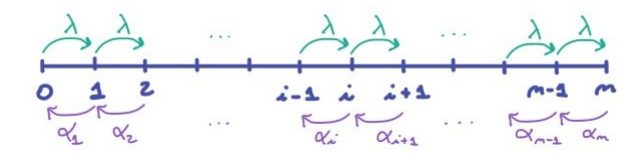
\includegraphics[width=0.75\textwidth]{diagrama_de_las_tasas_de_transicion}
\end{center}
para ciertos valores $\alpha_1, \alpha_2, \dots, \alpha_n$.
\begin{enumerate}[label=\roman*.]
	\item Hallar la probabilidad de que el primer cliente en arribar al sistema encuentre exactamente $k$ servidores ocupados (es decir, que al instante en el que arriba el primer cliente, el proceso $(X_t)_{t \geq 0}$ pase de $k$ a $k + 1$).
	\item Hallar la probabilidad de que el primer cliente en arribar al sistema encuentre exactamente $i$ servidores ocupados, con $i \in S$.
(Pensar primero el caso $i = k - 1$, $i = k - 2$, ect.)
	\item Hallar el número esperado de servidores ocupados que encuentra el primer cliente que arriba al sistema.
\end{enumerate}
\end{exercise}

%%%%%%%%%%%%%%%%%%%%%%%%%%%%%%
\begin{exercise}
Sea $(B_t)_{t \geq 0}$ un Movimiento Browniano estándar en dimensión 1.

Para cada $x \in \realnum$ sea $T_x = \inf \{t \geq 0 : B_t = x\}$.
(Notar que \(T_0 = 0\) a.s.)
Denotamos con \(f_{T_x}\) y \(F_{T_x}\) a la función de densidad y a la función de distribución acumuladad de \(T_x\), respectivamente.
\begin{enumerate}[label=\alph*)]
	\item Probar que \(\prob(T_x < + \infty) = 1\) para todo \(x \in \realnum\).
	(Sugerencia: puede ser útil observar el \(\sup_{t \geq 0} B_t\) y el \(\inf_{t \geq 0} B_t\))
	\item Para cada \(x \in \realnum \setminus \{0\}\), calcular \(f_{T_x}\) y verificar que \(\Exp(T_x) = + \infty\).
\end{enumerate}
\end{exercise}

%%%%%%%%%%%%%%%%%%%%%%%%%%%%%%
\begin{exercise}
Sea \((B_t)_{t \geq 0}\) un Movimiento Browniano estándar en dimensión 1, y sean \(x > 0\), \(y > 0\).
Consideremos el stopping time \(T = T_{- y} \wedge T_x\).
\begin{itemize}
	\item Probar que \((B_t^2 - t)_{t \geq 0}\) es una martingala.
	\item Probar que \(\Exp(T) = xy\)
\end{itemize}
\end{exercise}

%%%%%%%%%%%%%%%%%%%%%%%%%%%%%%
\begin{exercise}
(Este ejercicio no es obligatorio)

Sea \((B_t)_{t \geq 0}\) un Movimiento Browniano estándar en dimensión 1, y sean \(a > 0\), y \(b > 0\).
El objetivo es probar que \(\prob(B_t = a + b t \text{ para algún } t > 0) = e^{- 2 a b}\).
\begin{enumerate}[label=\alph*)]
	\item Sea \((X_t)_{t \geq 0}\) el proceso definido por \(X_t = e^{2 b B_t - 2 b^2 t}\).
	Probar que \((X_t)_{t \geq 0}\) es una martingala.
	\item Consideremos el stopping time \(T = \inf \{t > 0 : B_t = a + b t\}\) (donde \(T\) lo definimos como \(\infty\) si ese conjunto es vacío, es decir, si \(B_t < a + b t\) para todo \(t > 0\)).
	Probar que \(\Exp(X_T) \characteristic_{T < \infty} = 1\).
	\item Probar que \(\Exp(X_T \characteristic_{T < \infty}) = e^{2 a b} \prob(T < \infty)\).
	\item Concluir que \(\prob(B_t = a + b t\text{ para algún } t > 0) = e^{- 2 a b}\).
\end{enumerate}
\end{exercise}







\end{document}
